%; whizzy chapter -dvi
% -initex iniptex -latex platex -format platex -bibtex jbibtex -fmt fmt
% 以上 whizzytex を使用する場合の設定。
 
%     Tokyo Debian Meeting resources
%     Copyright (C) 2012 Junichi Uekawa
%     Copyright (C) 2011, 2015 Nobuhiro Iwamatsu

%     This program is free software; you can redistribute it and/or modify
%     it under the terms of the GNU General Public License as published by
%     the Free Software Foundation; either version 2 of the License, or
%     (at your option) any later version.

%     This program is distributed in the hope that it will be useful,
%     but WITHOUT ANY WARRANTY; without even the implied warranty of
%     MERCHANTABILITY or FITNESS FOR A PARTICULAR PURPOSE.  See the
%     GNU General Public License for more details.

%     You should have received a copy of the GNU General Public License
%     along with this program; if not, write to the Free Software
%     Foundation, Inc., 51 Franklin St, Fifth Floor, Boston, MA  02110-1301 USA

%  preview (shell-command (concat "evince " (replace-regexp-in-string "tex$" "pdf"(buffer-file-name)) "&"))

%%ここからヘッダ開始。

\documentclass[mingoth,a4paper]{jsarticle}
\usepackage{monthlyreport}
% 日付を定義する、毎月変わります。
\newcommand{\debmtgyear}{2015}
\newcommand{\debmtgmonth}{3}
\newcommand{\debmtgdate}{7}
% started from zero:
% (let ((year 2013) (month 7)) (+ (* (- year 2005) 12) month -1))
\newcommand{\debmtgnumber}{124}

\begin{document}

\begin{titlepage}
\thispagestyle{empty}
% タイトルページ:編集必要な部分は最初のマクロに飛ばすこと

\vspace*{-2cm}
第\debmtgnumber{}回 東京エリア Debian 勉強会資料\\
\hspace*{-2cm}

\includegraphics{image2012-natsu/dotdeb.pdf}\\
\hfill{}\debmtgyear{}年\debmtgmonth{}月\debmtgdate{}日

% ここはアップデートすること
% 全角文字にしないとフォントのサイズが合わないので注意
\rotatebox{10}{\fontsize{30}{30} {\gt 特集:ラズパイ 2 に Debian}}\\

\vspace*{-2cm}
\hfill{}
\includegraphics[height=6cm]{image200502/openlogo-nd.eps}
\end{titlepage}

\newpage

\begin{minipage}[b]{0.2\hsize}
 \definecolor{titleback}{gray}{0.9}
 \colorbox{titleback}{\rotatebox{90}{\fontsize{80}{80} {\gt デビアン勉強会} }}
\end{minipage}
\begin{minipage}[b]{0.8\hsize}
\hrule
\vspace{2mm}
\hrule
\begin{multicols}{2}
\tableofcontents
\end{multicols}
\vspace{2mm}
\hrule
\end{minipage}

\dancersection{事前課題}{野島 貴英}

今回の事前課題は以下です:
\begin{enumerate}
\item 本日、何の作業をやるかを宣言ください。
\item (オプション) どこで今回の勉強会の開催を知りましたか?
\item (オプション) 何について聞きたい/参加者と話をしたいですか?
\end{enumerate}
この課題に対して提出いただいた内容は以下です。
\begin{multicols}{2}
{\small
\begin{prework}{ $BLnEg(B }
  \begin{enumerate}
  \item Q.hack time$B$K2?$r$7$^$9$+!)(B\\
    A. DDTSS$B$7$^$C$9(B!\\
    http://ddtp.debian.net/ddtss/index.cgi/ja
  \item ($B%*%W%7%g%s(B)Q.$B2?$K$D$$$FJ9$-$?$$!?;22C<T$HOC$r$7$?$$$G$9$+!)(B\\
    A. $B;22C<T$H5;=Q$NOC$r$7$?$$!*(B
  \end{enumerate}
\end{prework}

\begin{prework}{ nametake }
  \begin{enumerate}
  \item Q.hack time$B$K2?$r$7$^$9$+!)(B\\
    A. Debian$B3+H/4D6-%;%C%H%"%C%W(B
  \item ($B%*%W%7%g%s(B)Q.$B$I$3$G:#2s$NJY6/2q$N3+:E$rCN$j$^$7$?$+!)(B\\
    A. $B$=$NB>!#(B
  \end{enumerate}
\end{prework}

\begin{prework}{ NOKUBI Takatsugu }
  \begin{enumerate}
  \item Q.hack time$B$K2?$r$7$^$9$+!)(B\\
    A. OpenCV$B!"(BKAKASHI$B!"(BBlender
  \item ($B%*%W%7%g%s(B)Q.$B$I$3$G:#2s$NJY6/2q$N3+:E$rCN$j$^$7$?$+!)(B\\
    A. $B$=$NB>(B
  \item ($B%*%W%7%g%s(B)Q.$B2?$K$D$$$FJ9$-$?$$!?;22C<T$HOC$r$7$?$$$G$9$+!)(B\\
    A. key sign
  \end{enumerate}
\end{prework}

\begin{prework}{ alohaug }
  \begin{enumerate}
  \item Q.hack time$B$K2?$r$7$^$9$+!)(B\\
    A. $B%/%j!<%s%k!<%`4D6-$G(BPGP$B80:n@.!"(BGnuk$BIuF~(B \& dictoss$B$5$s80=pL>(B
  \item ($B%*%W%7%g%s(B)Q.$B$I$3$G:#2s$NJY6/2q$N3+:E$rCN$j$^$7$?$+!)(B\\
    A. twitter (@tokyodebian)
  \item ($B%*%W%7%g%s(B)Q.$B2?$K$D$$$FJ9$-$?$$!?;22C<T$HOC$r$7$?$$$G$9$+!)(B\\
    A. PGP$B804IM}$N$"$k$"$k%M%?<}=8!#(B
  \end{enumerate}
\end{prework}

\begin{prework}{ kenhys }
  \begin{enumerate}
  \item Q.hack time$B$K2?$r$7$^$9$+!)(B\\
    A. $BL$Dj(B
  \item ($B%*%W%7%g%s(B)Q.$B$I$3$G:#2s$NJY6/2q$N3+:E$rCN$j$^$7$?$+!)(B\\
    A. Debian JP$B$N%a!<%j%s%0%j%9%H(B
  \end{enumerate}
\end{prework}

\begin{prework}{ Roger Shimizu }
  \begin{enumerate}
  \item Q.hack time$B$K2?$r$7$^$9$+!)(B\\
    A. $BL$Dj(B
  \item ($B%*%W%7%g%s(B)Q.$B$I$3$G:#2s$NJY6/2q$N3+:E$rCN$j$^$7$?$+!)(B\\
    A. $B$=$NB>(B
  \item ($B%*%W%7%g%s(B)Q.$B2?$K$D$$$FJ9$-$?$$!?;22C<T$HOC$r$7$?$$$G$9$+!)(B\\
    A. GPG$B%-!<%5%$%s$,9T$o$l$k$G$7$g$&$+!#(B
  \end{enumerate}
\end{prework}

\begin{prework}{ ryo\_s }
  \begin{enumerate}
  \item Q.hack time$B$K2?$r$7$^$9$+!)(B\\
    A. $B=q@RFI$_(B
  \item ($B%*%W%7%g%s(B)Q.$B$I$3$G:#2s$NJY6/2q$N3+:E$rCN$j$^$7$?$+!)(B\\
    A. $BM'C#$dCN$j9g$$$+$iD>@\(B
  \end{enumerate}
\end{prework}

\begin{prework}{ dictoss }
  \begin{enumerate}
  \item Q.hack time$B$K2?$r$7$^$9$+!)(B\\
    A. rasbbery pi 2$B$K(BDebian$B$r%$%s%9%H!<%k$9$k2<D4$Y!#(B
  \item ($B%*%W%7%g%s(B)Q.$B$I$3$G:#2s$NJY6/2q$N3+:E$rCN$j$^$7$?$+!)(B\\
    A. Debian JP$B$N%a!<%j%s%0%j%9%H(B
  \item ($B%*%W%7%g%s(B)Q.$B2?$K$D$$$FJ9$-$?$$!?;22C<T$HOC$r$7$?$$$G$9$+!)(B\\
    A. CPU$B$N%]!<%F%#%s%0$O2?$rCN$C$F$$$kI,MW$,$"$k$N$+65$($F2<$5$$!#(B
  \end{enumerate}
\end{prework}

\begin{prework}{ myokoym }
  \begin{enumerate}
  \item Q.hack time$B$K2?$r$7$^$9$+!)(B\\
    A. deb$B%Q%1!<%8$N:n@.<j=g$r0l$+$i3X$S$?$$$H;W$$$^$9!#(B
  \item ($B%*%W%7%g%s(B)Q.$B$I$3$G:#2s$NJY6/2q$N3+:E$rCN$j$^$7$?$+!)(B\\
    A. Debian JP$B$N%a!<%j%s%0%j%9%H(B
  \item ($B%*%W%7%g%s(B)Q.$B2?$K$D$$$FJ9$-$?$$!?;22C<T$HOC$r$7$?$$$G$9$+!)(B\\
    A. deb$B%Q%C%1!<%8$N:n@.$d8x3+$K$D$$$F(B
  \end{enumerate}
\end{prework}

\begin{prework}{ yy\_y\_ja\_jp }
  \begin{enumerate}
  \item Q.hack time$B$K2?$r$7$^$9$+!)(B\\
    A. DDTSS 
  \item ($B%*%W%7%g%s(B)Q.$B$I$3$G:#2s$NJY6/2q$N3+:E$rCN$j$^$7$?$+!)(B\\
    A. $B$=$NB>(B
  \item ($B%*%W%7%g%s(B)Q.$B2?$K$D$$$FJ9$-$?$$!?;22C<T$HOC$r$7$?$$$G$9$+!)(B\\
    A. DDTSS$B$N%l%S%e!<$N$*4j$$(B
  \end{enumerate}
\end{prework}



}
\end{multicols}

\dancersection{Debian Trivia Quiz}{野島 貴英}

 Debianの昨今の話題についてのQuizです。

今回の出題範囲は\url{debian-devel-announce@lists.debian.org} や \url{debian-news@lists.debian.org}に投稿された
内容などからです。

\begin{multicols}{2}
%; whizzy-master ../debianmeetingresume201311.tex
% $B0J>e$N@_Dj$r$7$F$$$k$?$a!"$3$N%U%!%$%k$G(B M-x whizzytex $B$9$k$H!"(Bwhizzytex$B$,MxMQ$G$-$^$9!#(B
%

\santaku
{2015/3/3$B$K(BDebConf15$B$N%"%J%&%s%9$,9T$o$l$^$7$?!#%9%]%s%5!<%I$J;22C$NEPO?4|8B$O2?;~$^$G$G$7$g$&!)(B}
{2015/3/7}
{2015/3/15}
{2015/3/29}
{C}
{$B=IGqBe$H?);v$,(BDebConf$B3+:EB&;}$A$H$J$k%9%]%s%5!<%I$J;22CEPO?$N!:@Z$O(B3/29$B$G$9!*!:@Z$N;~9o$O(BUTC$B$J$N$+!"%I%$%D$N%m!<%+%k%?%$%`$+!":Y$+$$;v$,$o$+$i$J$$$N$G!";22C$r8!F$$5$l$F$$$kJ}$O!:@Z$KBP$7$F==J,$KF|Dx$NM>M5$r$b$C$FEPO?$5$l$k;v$r$*$9$9$a$7$^$9!#(BDebConf15$B$O!"%I%$%D(B $B%O%$%G%k%P!<%0$G(B2015/8/15-22$B$N3+:E$G$9!#(BDebCamp$B$O!"(B8/9-8/14$B$H$J$j$^$9!#(B}

\santaku
{2015/3/4$B$K(BDPL$B$N:#G/$NA*=P$K$D$$$F%"%J%&%s%9$,$"$j$^$7$?!#(BDPL$B$NN)8uJd!:@Z$O2?;~!)(B}
{2015/3/4}
{2015/3/9}
{2015/4/1}
{B}
{$BKhG/91Nc$N(BDPL$BA*5s$G$9!#(BDPL$B$NN)8uJd!:@Z$O(B3/9$B$G!"A*5s$O(B4/1$B$+$i9T$o$l$^$9!#:#G/$OC/$,N)8uJd$9$k$N$G$7$g$&$+!)$^$?!"F1;~$K!"(BDebian JP Project$B$K$D$$$F$b!"(B2015$BG/$N2qD9$NN)8uJd<TJg=8$,9T$o$l$F$$$^$9!#(B}

\santaku
{2015/3/1$B$K$F!"(BAraki$B$5$s$h$j!"(B2007$BG/$+$i2TF/$7$F$$$?(Bcdn.debian.net$B$,$=$NLr3d$r=*$(!"$"$k(BFQDN$B$r;X$9$@$1$K$J$k$H$$$&$3$H$,%"%J%&%s%9$5$l$^$7$?!#$3$N(BFQDN$B$O0J2<$N$I$l!)(B}
{ftp.debian.org}
{http.debian.net}
{sources.debain.net}
{B}
{cdn.debian.net$B$O!"(Bapt$B$K$h$k(BDebian$B%Q%C%1!<%8$N<hF@@h$K$D$$$F!"(BDNS$B%/%(%j$NH/9T$5$l$?>l=j$K4p$E$$$F!"%f!<%6$K:G$b6a$$%Q%C%1!<%8%j%]%8%H%j$N%5!<%P$N(BIP$B%"%I%l%9$r(BDNS$B$N%l%3!<%I$GJV5Q$9$k;EAH$_$G$9!#(BAraki$B$5$s$K$h$C$F@_7W!"9=C[!"1?MQ$5$l$F$*$j$^$7$?!#(B2010$BG/$K(Bapt$B$,(BHTTP $B%j%@%$%l%/%H$r%5%]!<%H$G$-$k$h$&$K$J$C$?$?$a!"(Bcdn.debian.net$B$N5!G=$r(BHTTP$B$N%j%@%$%l%/%H5!G=$G<B8=$9$k(Bhttp.debian.net$B$,1?MQ$5$l$F$-$^$7$?!#:#2s!"?k$K!"(Bcdn.debian.net$B$r0zB`$5$;$k%"%J%&%s%9$,9T$o$l$?$H$$$&>u67$G$9!#$b$7!"(Bsource.list$B$K(Bcdn.debian.net$B$N(BFQDN$B$r;XDj$7$F$$$k>l9g$O!"(Bhttp.debian.net$B$KJQ$($^$7$g$&!#(B}



\end{multicols}

\dancersection{最近のDebian関連のミーティング報告}{野島 貴英}

\subsection{第123回東京エリアDebian勉強会}

\begin{itemize}
\item 場所はスクウェア・エニックスさんのセミナルームをお借りしての開催でした。
\item 参加者は9名でした。
\item セミナ内容は杉本さんによる「Debian GNU/kFreeBSDにおけるJail構築を試してみた」でした。
\item LTは、今井さんによる「Gnukと私」でした。
\item 残りの時間でhack timeを行い、成果発表をしました。
\item 「世界のやまちゃん 新宿花園店」で、久々に宴会をやりました。
\end{itemize} 

 セミナですが、kFreeBSD使いの杉本さんにより、Debian GNU/kFreeBSD上のJail環境で、
\begin{itemize}
\item GNU/kFreeBSD
\item FreeBSD 10.1-RELEASE
\end{itemize}
を動かすことについて発表がありました。さらに、FreeBSDの持つLinuxバイナリ互換機能でlinux-i386を動かすことにチャレンジされていました。linux-i386はうまくJail環境では動作しなかったとのことですが、試みとしては大変おもしろく、他では類を見ないものだったと思います。当勉強会では、うまくいった事も、うまくいかなかった事も、オリジナルな内容であれば、とても面白い話題となると考えています。今後も奇抜なアイデアの発表が当勉強会でどんどん発表されると良いですね!

 また、LTとして、今井さんにより、Gnuk Tokenについて語っていただきました。途中、1990年代のインターネット界隈と秋葉原での、関係者らの数々の偉業の話が多数飛び出すなど非常に刺激的な内容でした。また、何故専用ハードに秘密鍵を保管するのか?保管すべきなのか?についても情熱的に語っていただきました。Gnuk Tokenは、オープンなハード、オープンなソフトを使った、真にセキュアで真に自由な環境を手に入れることが出来るということについて、大変良い事例だと思います。Gunk Tokenを使うのが普通の世の中に早くなって欲しいものです。

\subsection{OSC 2015 Tokyo/spring出展} 

 毎年のことですが、今年も2/28(土)にて、OSC 2015 Tokyo/springが開かれました。
 場所はいつもの明星大学 日野キャンパスでした。セミナは、岩松さんにより「Debian Updates」が行われました。20名程度の方に来ていただけました。

 今回もブースを出展しました。今回の展示物としての目玉は、64bit ARM搭載の低価格ボードであるHikey Board(\url{https://www.96boards.org/products/hikey/})がDebian稼働状態で展示、また、Gnuk Tokenも展示されました。今回ブースの大きさが狭く、説明員が2名立つのがやっとというスペースでしたが、多くの人に立ち寄っていただけました。

 
% % (query-replace-regexp "<.*?>" "")
% % (query-replace-regexp "^[	 ]\+" "")

%-------------------------------------------------------------------------------
\dancersection{Raspberry Pi 2 Model B に Debian Jessie / armhf をインストールする}{岩松 信洋}
%-------------------------------------------------------------------------------
 \subsection{はじめに}

2015年2月2日に新しいRaspberry Pi「Raspberry Pi 2 Model B」が発売されました。
今回のRaspberry Pi 2(以下、RPi2)は今までのRaspberry Pi(RPi)とは異なり、SoC がアップグレード
されたものになっています。FPU を持っているにも関わらず Debian では armel をつかわなければ
なりませんでしたが、RPi2ではDebianのarmhf アーキテクチャが利用できるようになります。

本資料では Debianから見たRPi と RPi2 の違いと、RPi2 に Debian Jessie / armhf をインストール
する方法について紹介します。

\subsection{RPi と RPi2 の違い}

\begin{figure}[htbp]
\begin{center}
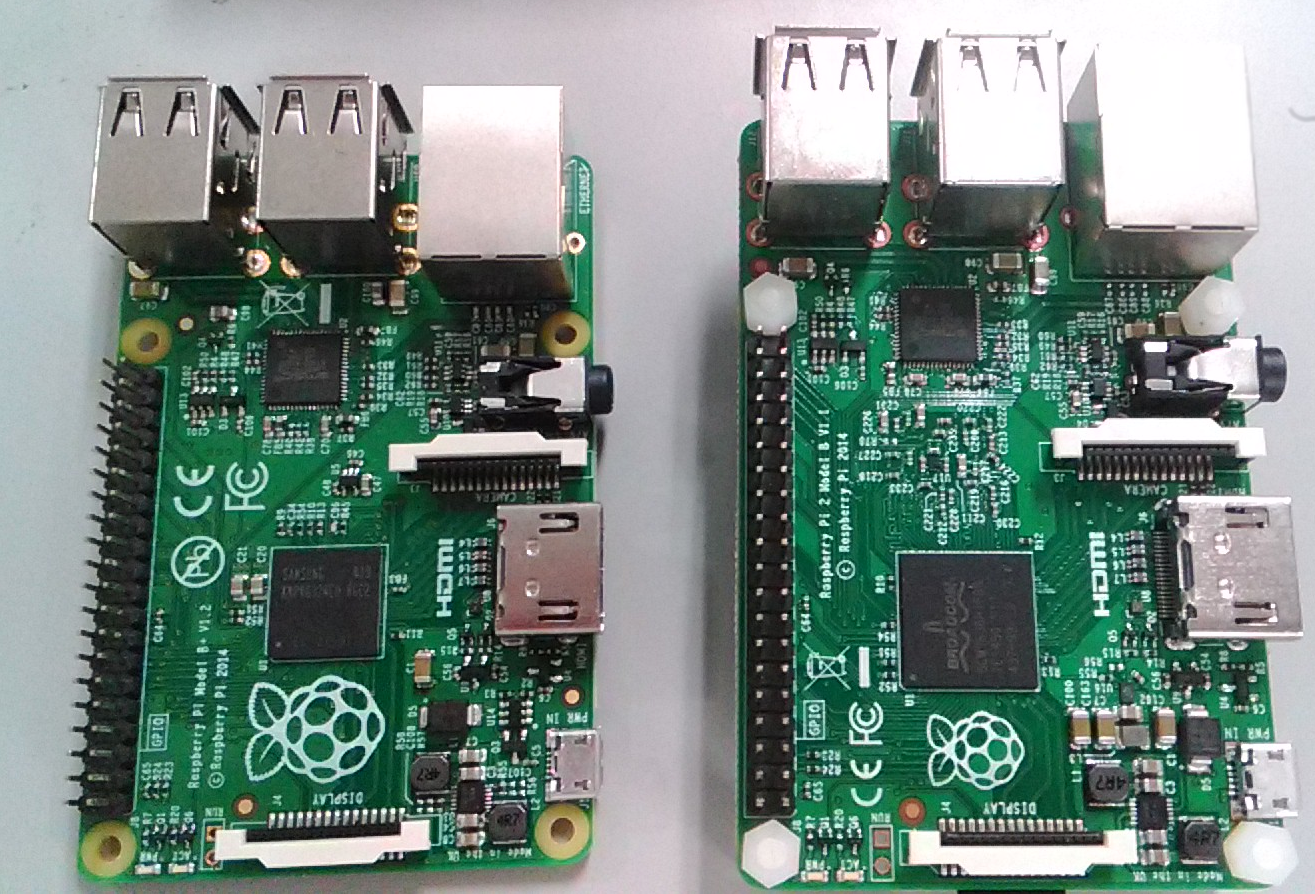
\includegraphics[width=0.7\hsize]{image201503/rpis.png}
\end{center}
\caption{RPi Model B+(左) とRPi 2 Model B(右)}
\label{fig:rpis}
\end{figure}

RPi (Model B+) とRPi 2 Model B のハードウェアは
表\ref{rpi-hw}となります。CPU、コア数、メモリの種類とサイズが大きく異なる
事が分かります。RPi2 ではコア数が増えているため、電源も大きめのものが必要
になっていることも注目すべき点です。
\begin{table}
\caption{RPi とRPi 2 B}
\begin{center}
\begin{tabular}{|c|c|c|}
\hline
-   & RPi Model B+ & RPi 2 Model B \\
\hline
CPU  & ARM1176JZF-S 1コア (700MHz) / ARMv6 & ARM Cortex-A7 4コア (900MHz) / ARMv7\\
SoC  & Broadcom BCM2835 &  Broadcom BCM2836 \\  
CPU  & Broadcom VideoCore IV (250MHz) & 同左 \\
メモリ & 512MB (SDRAM)& 1GB (LPDDR2 SDRAM) \\
ネットワーク & LAN9514 (10/100 Mbps) & 同左 \\
外部I/O & GPIO 40ピン & 同左 \\
ストレージ & microSD & 同左 \\
電源 & 600 mA (3.0W) & 900 mA (4.5-5.5W) \\
\hline
\end{tabular}
\label{fig:rpi-hw}
\end{center}
\end{table}

Debian armel、armhf、Raspbian の違いは表\ref{rpi-sw}の通りです。
各アーキテクチャでサポートする命令セットが異なり、Debian armel
では RPi/RPi2 に最適化されているとは言えないことがわかります。
Unixbench でベンチマークした結果を表\ref{rpi-bench}に示します。
RPi では Raspbian のよい結果となり、RPi2 では Debian / armhf が
よい結果となります。これは Raspbian が ARMv6 / VFPv2 に最適化
されたバイナリで、RPi2 に最適化されていないためです。
RPi2 では Raspbian より Debian / armhf を使ったほうが良いことが
わかりました。

\begin{table}
\caption{Debian と Raspbian}
\begin{center}
\begin{tabular}{|c|c|c|c|}
\hline`
 - & Debian armel & Debian armhf & Raspbian \\
\hline
ターゲット命令セット &  ARMv4 & ARMv7 & ARMv6 \\
FPU &  なし &  VFPv3  &  VFPv2 \\
Debian ネイティブ & Yes & Yes & No \\
\hline
\end{tabular}
\end{center}
\label{fig:rpi-sw}
\end{table}

\begin{table}
\caption{UnixBenchの結果}
\begin{center}
\begin{tabular}{|c|c|c|c|c|}
\hline`
 - & Debian armel / RPi & Debian armhf /RPi2 & Raspbian / Rpi & Raspbian / Rpi2 \\
\hline
Unixbench (System Benchmarks Index Score) & 66.5 & 450.8 (183.1) & 80.1 & 442.9 (173.8)\\
\hline
\end{tabular}
\end{center}
\label{fig:rpi-sw}
\end{table}


\subsection{Debian armhf / Jessie のインストール方法}

インストールには 実機、初期化されてもよい4GB以上のmicroSDカード、電源用の
micro USB ケーブル等が必要です。
またUSBシリアル変換モジュールがあるとコンソールから操作できるので、カスタマイズ
が楽にできます。接続例を図\ref{fig:rpi2-hw-setting}に示します。

\begin{figure}[htbp]
\begin{center}
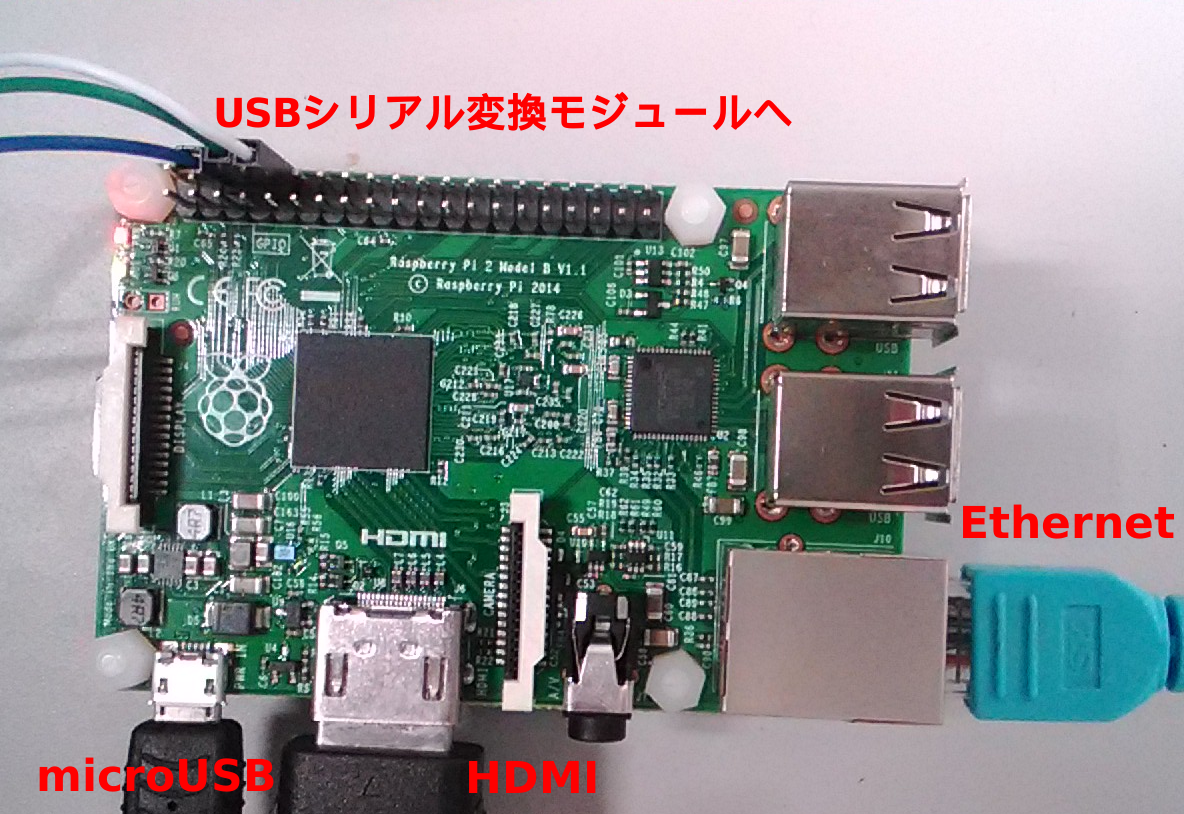
\includegraphics[width=0.7\hsize]{image201503/rpi2-hw-setting.png}
\end{center}
\caption{RPi2 接続例}
\label{fig:rpi2-hw-setting}
\end{figure}

またインストールの流れは以下となります。
\begin{enumerate}
\item microSDカードの認識確認
\item microSDカードの初期化
\item microSDカードにパーティション作成
\item microSDカードのフォーマット
\item cdebootstrap を使ってmicroSDカードにインストール
\item RPi2のLinuxカーネルとカーネルモジュールのインストール
\item RPi2のカーネルコマンドラインの設定
\item fstabの設定
\item ネットワークデバイスの設定
\item rootfs用パーティションの変更
\item root のパスワードの設定とrpiユーザの追加
\item microSDカードのアンマウントとRPi2の起動
\item RPi2 へのログイン
\item RPi2 専用ツールのインストール
\end{enumerate}

\subsubsection{microSDカード の接続確認}

使用している Debianに micorSD カードを挿入します。挿入するとdmesgに以下のような
メッセージが出力されるはずです。これでmicroSDがどのデバイスファイルに割り当てられた
かわかります。図\ref{fig:microsd}では sde に割り当てられていることがわかります。

\begin{figure}[htbp]

\begin{commandline}
$ dmesg  | tail -5
[858983.896718] FAT-fs (sdf1): Directory bread(block 32775) failed
[858983.896729] FAT-fs (sdf1): Directory bread(block 1390704) failed
[858983.896731] FAT-fs (sdf1): Directory bread(block 1390705) failed
[869873.800361] sd 6:0:0:3: [sde] 15523840 512-byte logical blocks: (7.94 GB/7.40 GiB)
[869873.831121]  sde: sde1
\end{commandline}
\caption{microSDカードのデバイスファイル割り当て確認}
\label{fig:microsd}
\end{figure}

\subsubsection{microSDカードの初期化}

購入したばかりのmicroSDカードはVFAT等でフォーマットされています。
MBRがある領域を 0 で埋めて初期化します(fdisk コマンド等で丁寧にやってもよいです)。

\begin{figure}[htbp]
\begin{commandline}
$ sudo dd if=/dev/zero of=/dev/sde bs=1M count=1
\end{commandline}
\caption{microSDカードの初期化}
\label{fig:microsd-format}
\end{figure}

\subsubsection{microSDカードにパーティション作成}

fdisk コマンドを使って microSD カードにパーティションを作成します。
図\ref{fig:createp}に手順を示します。
32MB、VFATで boot 用のパーティションを作成し、残りをrootfs 用にLinux 用に作成します。

一気にやりたい方は図\ref{fig:createp2} を実行すればよいです。

\begin{figure}[htbp]

\begin{commandline}
$ sudo fdisk /dev/sde
Command (m for help): o

Created a new DOS disklabel with disk identifier 0x9aa4e1fa.

Command (m for help): n
Partition type
   p   primary (0 primary, 0 extended, 4 free)
   e   extended (container for logical partitions)
Select (default p): p
Partition number (1-4, default 1): 1
First sector (2048-15523839, default 2048): 
Last sector, +sectors or +size{K,M,G,T,P} (2048-15523839, default 15523839): +32M

Created a new partition 1 of type 'Linux' and of size 32 MiB.

Command (m for help): t
Selected partition 1
Hex code (type L to list all codes): e
If you have created or modified any DOS 6.x partitions, please see the fdisk documentation for additional information.
Changed type of partition 'Linux' to 'W95 FAT16 (LBA)'.

Command (m for help): n
Partition type
   p   primary (1 primary, 0 extended, 3 free)
   e   extended (container for logical partitions)
Select (default p): p
Partition number (2-4, default 2): 2
First sector (67584-15523839, default 67584): 
Last sector, +sectors or +size{K,M,G,T,P} (67584-15523839, default 15523839): 

Created a new partition 2 of type 'Linux' and of size 7.4 GiB.

Command (m for help): w
The partition figure has been altered.
Calling ioctl() to re-read partition figure.
Syncing disks.
\end{commandline}

\caption{microSDカードにパーティションを作成}
\label{fig:createp}
\end{figure}

\begin{figure}[htbp]
\caption{microSDカードにパーティションを作成 一気にやるバージョン}
\begin{commandline}
(echo o; echo n; echo p; echo 1; echo ; echo +32M; echo t; echo e; echo n; echo p; echo 2; echo ; echo ; echo w) | fdisk /dev/sde
\end{commandline}
\label{fig:createp2}
\end{figure}

\subsubsection{microSDカードのフォーマット}

パーティション1 は mkfs.msdos で、パーティション2 は mkfs.ext でフォーマットします。
フォーマットできたら適当なディレクトリを作成し、2つのパーティションをマウントします。
今回は パーティション1用に /tmp/boot ディレクトリ、パーティション2用
に/tmp/rootfs ディレクトリを作成し、マウントします。

\begin{figure}[htbp]
\begin{commandline}
$ sudo mkfs.msdos /dev/sde1
$ sudo mkfs.ext4 /dev/sde2
$ mkdir /tmp/boot /tmp/rootfs
$ sudo mount /dev/sde1 /tmp/boot
$ sudo mount /dev/sde2 /tmp/rootfs
\end{commandline}
\caption{microSDカードのフォーマットとマウント}
\label{fig:microsdformat}
\end{figure}

\subsubsection{cdebootstrap を使ってmicroSDカードにインストールする}

cbootstrap を使って、microSDカードに debian 起動イメージをインストールします。
操作しているマシンがPC(i386やamd64)の場合、通常はarmhf
のバイナリを実行できません。そのためPC等で先にインストールに必要なDebianパッケージのダウンロード
と展開を行い、実際のインストールは RPi2 で行うという方法を取ります。
実際のインストール方法は図\ref{fig:firstbootstrap}となります。今回のインストールでは standard で
指定されているパッケージの他、シリアルコンソールが使えない環境を考えopenssh-server、
時間設定のためにntp、証明書のためにca-certificates、エディタとしてvimをインストールするようにして
います。もし他に一緒にインストールしたいパッケージがある場合は {\bf $-$$-$include} に続けて指定する事ができます。

\begin{figure}[htbp]
\begin{commandline}
$ sudo cdebootstrap --arch=armhf -f standard --foreign jessie \
  --include=openssh-server,ntp,ca-certificates,vim /tmp/rootfs
...
\end{commandline}
\caption{cdebootstrapを使ったDebianイメージのインストール}
\label{fig:firstbootstrap}
\end{figure}

\subsubsection{RPi2のLinuxカーネルとカーネルモジュールのインストール}

残念なことにRPi2のLinuxカーネルはDebianでは提供されていません。その理由として
まだ完全にアップストリームでサポートされていない事と起動にファームウェアが
必要ということが挙げられます。Debianで RPi2 のLinuxカーネルを扱うにはrpi-update
というツールを使う必要があります。

図\ref{fig:kernelinstall}ではrpi-update をRPi2 のrootfs にダウンロードした後、
実行権限を付加し、rpi-update を使ってカーネルとカーネルモジュールをインストールします。

\begin{figure}[htbp]
\begin{commandline}
$ sudo curl -o /tmp/rootfs/usr/bin/rpi-update https://raw.githubusercontent.com/Hexxeh/rpi-update/master/rpi-update
$ sudo chmod +x /tmp/rootfs/usr/bin/rpi-update
$ sudo mkdir /tmp/rootfs/lib/modules
$ sudo ROOT_PATH=/tmp/rootfs BOOT_PATH=/tmp/boot /tmp/rootfs/usr/bin/rpi-update
*** Raspberry Pi firmware updater by Hexxeh, enhanced by AndrewS and Dom 
 *** Performing self-update
  % Total    % Received % Xferd  Average Speed   Time    Time     Time  Current
                                 Dload  Upload   Total   Spent    Left  Speed
100  8107  100  8107    0     0  54471      0 --:--:-- --:--:-- --:--:-- 54777
 *** Relaunching after update
...
\end{commandline}
\label{fig:kernelinstall}
\caption{rpi-updateのインストールとLinuxカーネルのインストール}
\end{figure}

\subsubsection{RPi2のカーネルコマンドラインの設定}

RPi2のカーネルコマンドラインを設定します。RPi は/boot/cmdline.txt
に記載されているカーネルコマンドラインを読み込んで起動します。
図\ref{fig:commandlineset}のように実行し、カーネルコマンドラインを設定します。

\begin{figure}[htbp]
\begin{commandline}
$ sudo sh -c "echo dwc_otg.lpm_enable=0 console=ttyAMA0,115200 console=tty1
     root=/dev/mmcblk0p2 rootwait > /tmp/boot/cmdline.txt
\end{commandline}
\label{fig:commandlineset}
\caption{カーネルコマンドラインの設定}
\end{figure}

\subsubsection{fstabの設定}

fstabの設定を行ないます。procfs、rootfs, boot ディレクトリの設定を記載します。

\begin{figure}[htbp]
\begin{commandline}
proc            /proc           proc    defaults	0	0
/dev/mmcblk0p1  /boot           vfat    defaults	0	2
/dev/mmcblk0p2  /               ext4    defaults,noatime	0	1
\end{commandline}
\label{fig:rpiconfig}
\caption{fstabの設定}
\end{figure}

\subsubsection{ネットワークデバイスの設定}

rootfs/etc/network/interfaces を編集し、ネットワークデバイスを有効にします。
この操作は必須ではありませんが、USBシリアル変換モジュールを持ってない人
はRPi2 にSSHでログインして操作する必要がありますので、ここでネットワークを
起動時に有効するように設定しておきます。
RPi2 のIPアドレスをDHCPから取得する場合は図\ref{fig:netinterfaces}のように設定します。

\begin{figure}[htbp]
\begin{commandline}
auto eth0
iface eth0 inet dhcp
\end{commandline}
\label{fig:netinterfaces}
\caption{ネットワークデバイスの設定}
\end{figure}

\subsubsection{rootfs用パーティションの変更}

rootfs/sbin/init に書かれている 2nd bootstrap の内容に
rootfs をマウントする行があります。デフォルトでは rootfs を / にマウントする
よう記述されているため、このままではインストールに失敗します。
正しくインストールできるように rootfs を /dev/mmcblk0p2 に変更します。

\begin{figure}[htbp]
\begin{commandline}
trap 'error "Interruped!"' HUP INT TERM

mount -n -o remount,rw rootfs / <- これを
mount -n -o remount,rw /dev/mmcblk0p2 / <- これに変更

chown -hR 0:0 /
\end{commandline}
\label{fig:rpiconfig}
\caption{ネットワークデバイスの設定}
\end{figure}

\subsubsection{root のパスワードの設定とrpiユーザの追加}

現状のままではインストール完了後にログインできません。
2nd bootstrap 時にroot のパスワードを設定する処理を追加します。
また rpiユーザを作成し、パスワードを設定する処理も追加します。
rpi ユーザは説明のために使っているだけですので、他のユーザ名でも問題ありません。

\begin{figure}[htbp]
\begin{commandline}
echo 'deb http://ftp.debian.org/debian jessie main' > /etc/apt/sources.list

echo "root:root" | chpasswd <- この行を追加
useradd -m rpi <- この行を追加
echo rpi:rpi | chpasswd <- この行を追加

run rm /sbin/init
\end{commandline}
\label{fig:rpiconfig}
\caption{root パスワードの設定}
\end{figure}

\subsubsection{microSDカードのアンマウントとRPi2の起動}

microSDカードをアンマウントし、PRi2 の microSDカードスロット
に挿入します。挿入後、micro USB ケーブルを RPi2 に挿し、
RPi2を起動します。起動すると自動的に2nd bootstrap が実行され、
RPi2上でインストールが実行されます。
もしHDMI接続ができるモニターを持っている場合は、RPi2 と接続すると
インストールされる様子を確認できます。
インストール完了まで30分ほど待たされるので、気長に待ちましょう。
HDMIが利用できるモニターを持ってない場合、インストールが完了したか
見た目ではわからないので、RPi2 にIPアドレスが割り当てられているか、ping を
実行して反応があるかなどで確認する必要があります。

\subsubsection{RPi2 へのログイン}

インストールが完了すると自動的に init が再実行され、Debian が立ち上がった状態になっています。
USBシリアルモジュール経由や、SSH経由でログインできるようになっていますので、ログインして
ください。後は通常のDebianと変わりません。

\subsubsection{RPi2 専用ツールのインストール}

RPi2 の専用ツールである rpi-update、raspi-config はまだDebianでは提供されていません。
これらはカーネルやファームウェアのアップデート、RPiハードウェアの設定を行うための機能が
搭載されており、RPi ユーザには必須のツールとなっています。
これを Debian で利用できるようにするには raspberrypi.org で提供されている 各ツールの
Debian パッケージをインストールする必要があります。
図\ref{fig:rpirep}に設定方法を示します。

\begin{figure}[htbp]
\begin{commandline}
# wget -O - http://archive.raspberrypi.org/debian/raspberrypi.gpg.key | apt-key add - 
# echo deb http://archive.raspberrypi.org/debian wheezy main >> /etc/apt/sources.list
# apt-get update
# apt-get install rpi-update raspi-config
\end{commandline}
\label{fig:rpirep}
\caption{rpi-config、rpi-update パッケージのインストール方法}
\end{figure}

\subsubsection{終わりに}

RPi2 から ネイティブのDebianが利用できるようになりました。
インストーラやmicroSDカードイメージが準備されていなくても、今回解説した方法を使うと
RPi2 に自分好みのDebianをインストールできるようになります。CPUも強化されそこそこ使い
やすくなった Rpi2 で Debianを触ってみてはいかがでしょうか。

%-------------------------------------------------------------------------------
\dancersection{会場での無線LANのつなぎ方}{野島 貴英,Roger}
%-------------------------------------------------------------------------------
 \subsection{はじめに}

 今回試験として、会場側でフィルタ無しのグローバル回線を用意しました。
ただ、会場側のセキュリティポリシーにより、wpa-psk AES hidden SSIDという
方式での提供となります。

 以下にDebianマシンでの接続方法を記載します。

 また、自分の環境では違うやり方でつながったという方は、野島まで
教えて下さい。こちらでもノウハウとして溜めていく予定です。

 \subsection{wpasupplicant及び/etc/network/interfacesを利用の場合}

 もっとも良いマニュアルは、/usr/share/doc/wpasupplicant/README.Debian.gz
となります。困った場合はこちらも合わせてご参照下さい。

 以下に/etc/network/interfacesの定義について会場の例を記載します。

\begin{commandline}
$ sudo vi /etc/network/interfaces
-----以下のエントリがなければ追記ここから----------
iface wlan0_debian inet dhcp
     wpa-conf /etc/wpa_supplicant/wpa_supplicant_debian.conf
-----以下のエントリがなければ追記ここまで----------
$ sudo vi /etc/wpa_supplicant/wpa_supplicant_debian.conf
-----以下のエントリを追記ここから----------
network={
     ssid=<<会場のSSID>>
     psk=<<会場のパスワード>>
     scan_ssid=1
}
-----以下のエントリを追記ここまで----------
$ sudo chmod 600 /etc/wpa_supplicant/wpa_supplicant_debian.conf
$ sudo ifup wlan0=wlan0_debian
\end{commandline}
%$

 また、ハマってしまった時のデバッグ方法は、
/usr/share/doc/wpasupplicant/README.Debian.gz中の''4. Trubleshooting''の章が便利です。

 \subsection{その他の無線LAN用パッケージを利用の場合}

 すみません、自分が情報を持たないため、現場で教えて下さい。

\cleartooddpage

\vspace*{15cm}
\hrule
\vspace{2mm}

\includegraphics[width=2cm]{image200502/openlogo-nd.eps}
\noindent \Large \bf Debian 勉強会資料\\
\noindent \normalfont \debmtgyear{}年\debmtgmonth{}月\debmtgdate{}日 \hspace{5mm}  初版第1刷発行\\
\noindent \normalfont 東京エリア Debian 勉強会 (編集・印刷・発行)\\
\hrule

\end{document}
